\documentclass[final]{beamer}

\usepackage[scale=1.35]{beamerposter}
\usetheme{confposter}

\usepackage[utf8]{inputenc}
\usepackage[T1]{fontenc}
\usepackage{libertine}
\usepackage[libertine]{newtxmath}
% \usepackage{graphicx}  % Required for including images
\usepackage{mwe}
\usepackage{pifont} % pro pekne znacky http://ctan.org/pkg/pifont
\newcommand{\cmark}{\ding{51}} % pekne znacky
\newcommand{\xmark}{\ding{55}} % pekne zncky§


% \usetheme{confposter} % Use the confposter theme supplied with this template

\setbeamercolor{block title}{fg=nred,bg=white} % Colors of the block titles
\setbeamercolor{block body}{fg=black,bg=white} % Colors of the body of blocks
\setbeamercolor{block alerted title}{fg=white,bg=dblue!70} % Colors of the highlighted block titles
\setbeamercolor{block alerted body}{fg=black,bg=dblue!10} % Colors of the body of highlighted blocks
\setlength{\topmargin}{-0.5in} % Reduce the top margin size

\title{\#filterbubble} % Poster title
\author[dostal.jakub@outlook.com]{F. Sandroni, J. Dostal} % Author(s)
\institute{Slavonic grammar school Olomouc} % Institution(s)

\begin{document}

\addtobeamertemplate{block end}{}{\vspace*{2ex}} % White space under blocks
\addtobeamertemplate{block alerted end}{}{\vspace*{2ex}} % White space under highlighted (alert) blocks
\setlength{\belowcaptionskip}{2ex} % White space under figures
\setlength\belowdisplayshortskip{2ex} % White space under equations

\begin{frame}[fragile]
\begin{columns}[T]
% #############################################################################
% #############################################################################
% #############################################################################
% First Column
\begin{column}{.33\textwidth}

\begin{block}{Filter Bubble}
    \center
    \begin{large}\textbf{Living in one's own information environment.}\end{large}
    \vspace{0.8cm}
    \begin{itemize}
        \item occures on social networks
        \item caused by preferential algorithms
        \item first mentioned by Eli Pariser (2011)
    \end{itemize}
\end{block}
% #############################################################################
\begin{block}{Twitter}
	\begin{itemize}
		\item microblogging platform
        \item \textbf{following, followers} system
		\item Twitter API is suitable data source
	\end{itemize}
	\center
	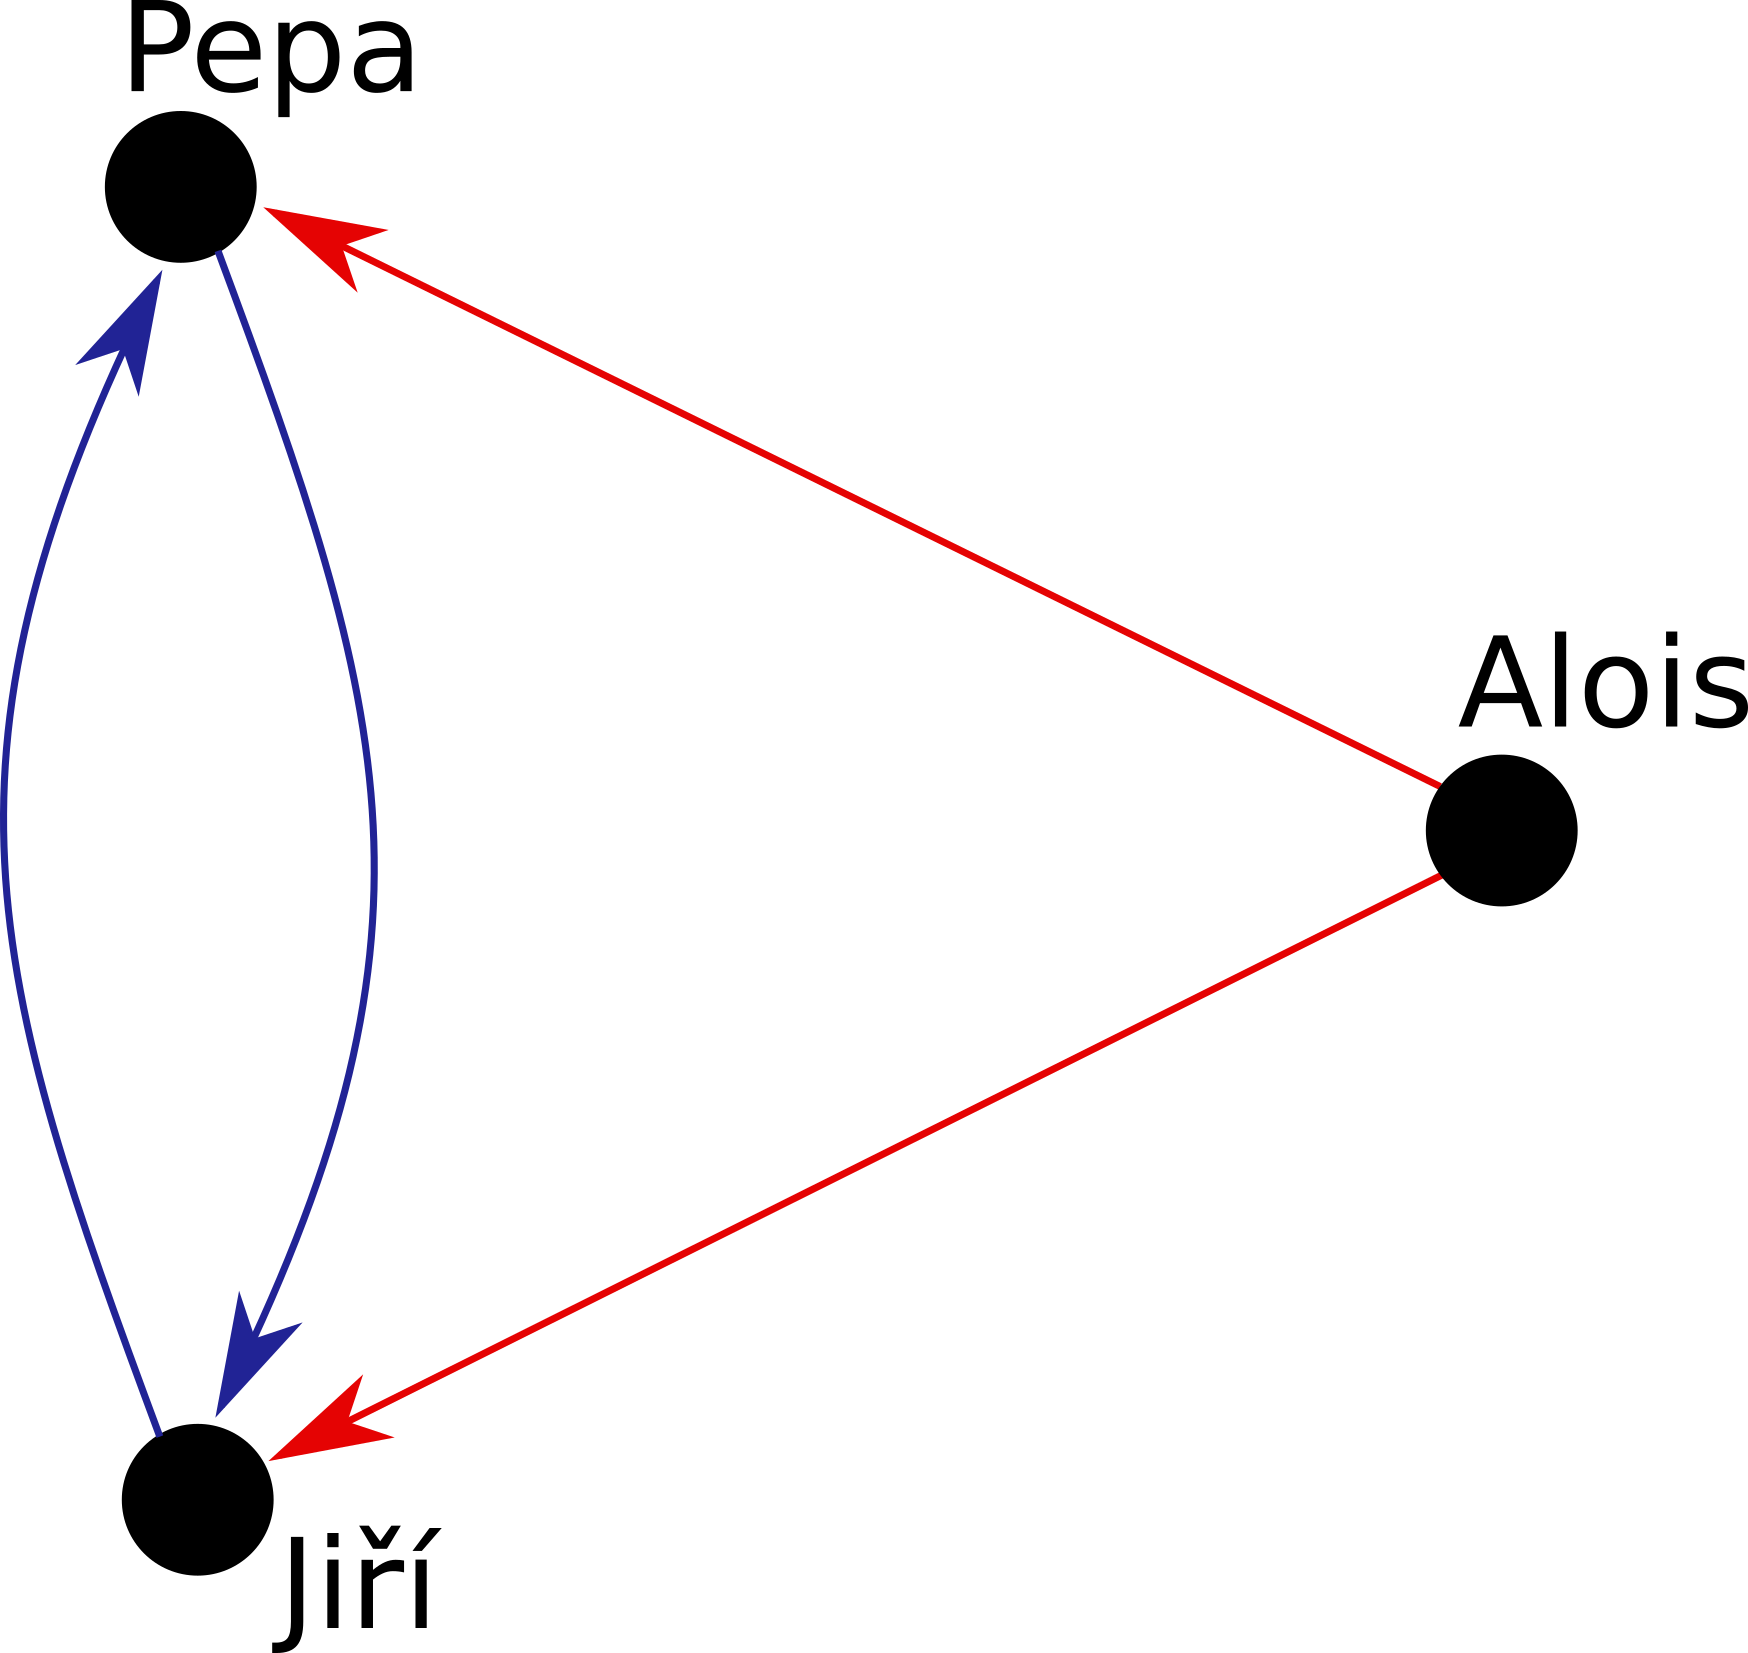
\includegraphics[scale=0.55]{./Pics/pepa.png}
\end{block}
% #############################################################################
\begin{block}{Studied groups selection}
    \begin{columns}
        \begin{column}{.5\textwidth}
            \begin{itemize}
                \item random sample from followers of the significant group
            \end{itemize}
        \end{column}
        \begin{column}{.5\textwidth}
            \center
            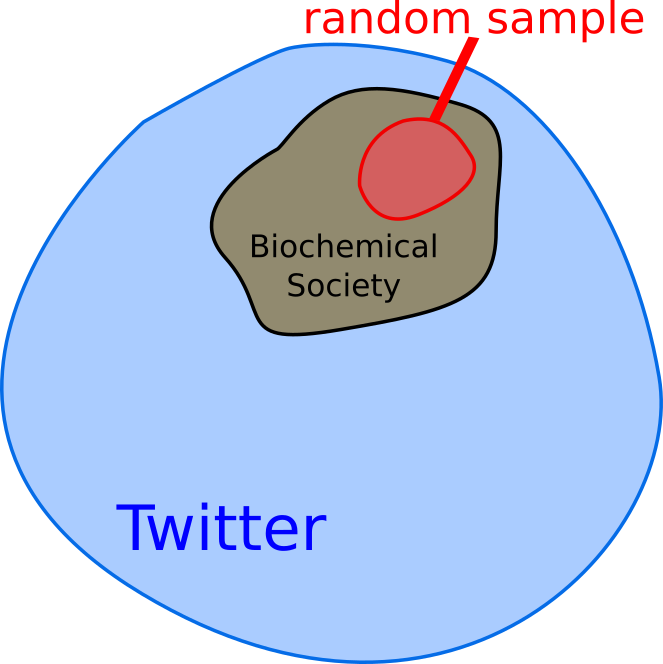
\includegraphics[scale=0.45]{./Pics/sets.png}
        \end{column}
    \end{columns}
    \center
    $\text{Twitter} \rightarrow \text{Biochemical Society} \rightarrow \text{\textbf{studied people}}$
\end{block}
% #############################################################################
\begin{block}{Tweets collection}
    \begin{columns}
    \column{.5\textwidth}
    	\begin{itemize}
            \item analysing content affecting the studied people
    	\end{itemize}
    \column{.5\textwidth}
    	\center
    	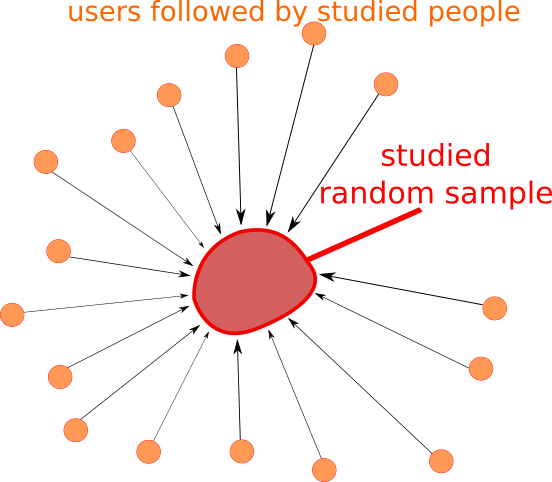
\includegraphics[scale=0.65]{./Pics/followers.png}
    \end{columns}
    \vspace{0.8cm}
    \begin{itemize}
        \item i. e. content from \textbf{followed people}
    \end{itemize}
\end{block}
% #############################################################################
\begin{block}{Tweets filtering}
\begin{itemize}
    \item filter only tweets on given topic
\end{itemize}
\vspace{0.3cm}
Keyword \textbf{"Trump"}:
\vspace{0.7cm}
\begin{itemize}\centering
    \item[\textcolor{black}{\xmark}] I had fish and chips for lunch.
    \item[\textcolor{black}{\cmark}] I'm glad Donald \textbf{Trump} is the president of the USA.
    % \item[\textcolor{black}{\xmark}] The president of the USA is a gentleman.
\end{itemize}
\end{block}
% #############################################################################
\begin{block}{Sentimental analysis}
\begin{itemize}
    \item measure sentiment of collected tweets
    \item \textbf{positive} vs. \textbf{negative} tweets
\end{itemize}
\center
\textit{Donald Trump is a terrible person.}\\
\textbf{(0.14)}\\
\vspace{0.5cm}
\textit{Donald Trump is a great person.}\\
\textbf{(0.95)}
\end{block}

\end{column}
% #############################################################################
% #############################################################################
% Second Column
\begin{column}{.63\textwidth}
    \begin{alertblock}{Motivation}
        \begin{columns}
            \begin{column}{.5\textwidth}
                \begin{large}\textbf{Threats for democracy:}\end{large}
                \vspace{0.5cm}
                \center
                content \textbf{homogeneity}\\
                $\Downarrow$\\
                loss of objectivity\\
                $\Downarrow$\\
                \textbf{radicalization}
            \end{column}
            \begin{column}{.5\textwidth}
                \begin{large}\textbf{Goals:}\end{large}
                \vspace{0.5cm}
                \begin{itemize}
                    \item filter bubble detection
                    \item filter bubble quantification
                \end{itemize}
            \end{column}
        \end{columns}
    \end{alertblock}
\end{column}
\end{columns}
% #############################################################################
% #############################################################################
% #############################################################################








% \begin{columns}[T]
% % #############################################################################
% % #############################################################################
% % #############################################################################
% % First Column
% \begin{column}{.33\textwidth}
%
% \end{column}
% % #############################################################################
% % #############################################################################
% % #############################################################################
% % Second Column
% \begin{column}{.3\textwidth}
%
% \end{column}
% % #############################################################################
% % #############################################################################
% % #############################################################################
% % Third column
% \begin{column}{.33\textwidth}
%
% \end{column}
% % #############################################################################
% % #############################################################################
% % #############################################################################
% \end{columns}

\end{frame}
\end{document}
